\documentclass[11pt, letterpaper]{article}
\usepackage[spanish]{babel}
\usepackage[utf8]{inputenc}
\usepackage{amsmath,amssymb,amsfonts}
\usepackage{enumerate}
\usepackage{subfig}
\usepackage{nicefrac}
\usepackage{url}
\usepackage{multirow}
\usepackage{graphicx}
\usepackage{setspace}

\usepackage[right=2.5cm, left=2.5cm, top=2cm, bottom=2cm]{geometry}

\decimalpoint

\begin{document}
% \maketitle

\thispagestyle{empty}

\noindent 
\begin{center}
  
\includegraphics[width=5em]{cebolla.png}\\
  Universidad Simón Bolívar\\
  Decanato de Estudios de Postgrado\\
  Postgrado en Ciencias de la Computación\\
  Representación del Conocimiento \\
  \vfill
  {\Huge Node splitting y MPE}
  \vfill
  Daniel Izquierdo \\
  Julio Castillo\\[2em]
  Julio de 2009
\end{center}

\newpage

\section{Introducción}

El problema MPE (\emph{most probable explanation}) consiste en averiguar, dadas
una red bayesiana y una evidencia, la instanciación más probable compatible con
la evidencia. Se ha propuesto \cite{Darwiche01alogical} una técnica de
compilación de redes bayesianas a circuitos aritméticos que permite cálculo
rápido del MPE. Sin embargo, la técnica está limitada a instancias de redes
pequeñas porque involucra un paso de compilación de una fórmula en CNF a su
equivalente en d-DNNF que puede tomar mucho tiempo con casos más grandes.

Por otra parte, existe un método para calcular cotas superiores del
MPE de redes bayesianas mediante eliminación de arcos
\cite{ChoiChaviraDarwiche07}. Es llamado \emph{node splitting} y
consiste básicamente en dividir nodos del grafo en dos y trasladar algunos
arcos salientes del nodo dividido al nodo creado en la división. Una
particularidad del método es que tras ser aplicado sobre redes bayesianas
grandes puede
reducir el tiempo de compilación a d-DNNF a magnitudes razonables. La
evaluación del MPE sobre un circuito aritmético generado por una red dividida
puede hacerse muy velozmente, y resulta en una cota superior para el MPE de la
red original con la misma evidencia.

Este documento describe brevemente una técnica
para calcular el MPE
de una red bayesiana grande utilizando como heurística la cota superior
proporcionada por el MPE de una red simplificada mediante \emph{node splitting}.
El cálculo del MPE en la red simplificada se realiza utilizando una
codificación en un circuito aritmético. Se produjo una implementación y se
ejecutó una serie de experimentos para evaluarla.

\section{Implementación}

\subsection{Cálculo de MPE utilizando teorías en d-DNNF}
\label{sec:condificacion}

Para comenzar definiremos el término de función multilineal, de central
importancia para este proyecto ya que codificaremos redes bayesianas como
funciones multilineales, a su vez codificadas como circuitos aritméticos
mediante el paso de traducción a d-DNNF. Una función es multilineal si es una
función aritmética de varias variables lineal en cada variable.

En nuestra implementación, una red bayesiana se convirtió a una teoría $\Delta$
en CNF de la
siguiente forma
\begin{itemize}
\item Para cada variable $X$ de la red bayesiana que toma valores
  $x^1,\dots,x^n$, se agregan a $\Delta$ las siguiente clausulas
  \begin{align}
    \lambda_{x^1} \lor \cdots \lor \lambda_{x^n} \label{eq:cnf1} \\
    \neg\lambda_{x^i} \lor \neg\lambda_{x^j} \quad i\neq j \label{eq:cnf2}
  \end{align}
\item Para cada variable $X$ con padres $U$, se crea una variable
  $\theta_{x|u_1,\dots,u_m}$, $\Delta$
  contiene:
  \begin{align}
    \lambda_{x} \land \lambda_{u_1} \land \cdots \land \lambda_{u_m} \Rightarrow \theta_{x|u_1,\dots,u_m} \label{eq::cnf3}\\
    \theta_{x|u_1,\dots,u_m} \Rightarrow \lambda_{x}, \;\; \theta_{x|u_1,\dots,u_m} \Rightarrow \lambda_{u_1} ,\;\; \dots \;\;, \theta_{x|u_1,\dots,u_m} \Rightarrow \lambda_{u_m} \label{eq:cnf4}
  \end{align}
\end{itemize}

Posteriormente $\Delta$ se compila a una teoría $\Gamma$
equivalente en d-DNNF smooth utilizando
\texttt{c2d}~{\cite{darwicheAAAI02}}. Luego en $\Gamma$ se sustituyen
los literales negativos por $1$, las conjunciones por
multiplicaciones y las disjunciones por sumas. Esta sustitución
permite hacer inferencia sobre la red bayesiana sustituyendo en
$\Gamma$ las variables $\theta$ por las probabilidades
correspondientes y las variables $\lambda_x$ por 1 si $x$ es
compatible con la evidencia o 0 si es imcompatible~\cite{Darwiche01alogical}.

Esta sustitución produce lo que se conoce como una representación en
circuito aritmético de la red bayesiana. Este circuito aritmético, al
evaluarlo de la forma indicada, corresponde a evaluar la función
multilineal asociada a la red bayesiana.

% Por ejemplo, para una red con variables $A$, $B$ y $C$, la función
% multilineal asociada es
% \begin{align}
%   f & = \lambda_a\lambda_b\lambda_c\
% \end{align}

Cada sumando en la función multilineal de una red corresponde a la
probabilidad de una instanciación particular compatible con la
evidencia. Si sustituimos las sumas por el operador $\max$,
obtendremos la asignación de variables de máxima probabilidad para una evidencia,
es decir, la probabilidad del MPE. Por lo tanto, si en $\Gamma$
sustituimos las disjunciones por $\max$, entonces podemos calcular el
MPE de la red utilizando el circuito aritmético.

\subsubsection{Restricciones Lógicas}
Una restricción lógica es una probabilidad condicional que es igual a
0 o 1. En cada uno de estos casos se pueden hacer simplificaciones
sobre $\Delta$ que permiten reducir significativamente el tamaño de la
teoría compilada en d-DNNF.

Si tenemos una red bayesiana con parámetro $\theta_{x|u_1,\dots,u_m}$
que toma valor cero, entonces las clausulas \eqref{eq::cnf3} y
\eqref{eq:cnf4} que involucran a $\theta_{x|u_1,\dots,u_m}$ se pueden sustituir por
\begin{equation}
  \label{eq:simpcero}
  \neg \lambda_{x} \lor \neg \lambda_{u_1} \lor \cdots \lor \neg \lambda_{u_m}
\end{equation}
Es decir, que $\theta_{x|u_1,\dots,u_m}$ se puede eliminar de
$\Delta$. Por otro lado, cuando $\theta_{x|u_1,\dots,u_m}=1$, podemos
omitir por completo a $\theta_{x|u_1,\dots,u_m}$ y las clausulas que
la mencionan.

Como se mostrará más adelante, estas simplificaciones tienen un gran
impacto sobre el tamaño de la teoría compilada cuando la red bayesiana
esta compuesta por una gran cantidad de nodos determinísticos (probabilidad 0 o
1).

% \subsubsection{Detalles de implementación}
% \label{sec:detall-de-impl}
% Para hacer la traducción a CNF primero se hace un mapeo 

\subsection{Cálculo de MPE para redes grandes}
\label{sec:calculo-de-mpe}
Para redes bayesianas con muchos nodos, el paso de compilación a
d-DNNF que se explicó anteriormente no termina en una tiempo
razonable. En este caso utilizamos la técnica de \textsl{node
  splitting} propuesta en~\cite{ChoiChaviraDarwiche07}.

La idea es tomar la red original y hacer una serie splittings (divisiones)
hasta
que sea posible compilar la red a d-DNNF y luego utilizar el MPE sobre
esta nueva red (que se puede calcular utilizando el circuito
aritmético) como heurística para obtener el MPE de la red original.

Este método se basa en el teorema~1 de \cite{ChoiChaviraDarwiche07} el
cual dice que si $N$ es un red bayesiana y $N'$ es el resultado de
hacer un splitting en $N$, entonces
\begin{equation}
  \label{eq:2}
  MPE_p(N,\mathbf{e}) \leq \beta MPE_p(N', \mathbf{e}, \vec{\mathbf{e}})
\end{equation}
donde $\vec{\mathbf{e}}$ es el conjunto de instanciaciones compatibles con $e$,
y $\beta = \prod_{C \in \mathbf{C}} |C|$ donde $\mathbf{C}$ es el conjunto de
clones en $N'$.

Si tenemos una red bayesiana $N'$ que es el resultado de hacer
splitting sobre la red $N$, entonces el procedimiento para calcular
$MPE(N,\mathbf{e})$ utilizando $N'$ se describe a continuación. Se
tiene una variable $\mathbf{z}$ que representa una asignación parcial
en $N$ y una segunda variable $q*$ que representa la cota inferior
actual para el MPE de de $N$. La búsqueda se inicia con $\mathbf{z} =
\mathbf{e}$ y $q* = 0$. En cada nodo del algoritmo de búsqueda
computamos $q$, una cota superior para el MPE de $N'$ y la
instanciación parcial $\mathbf{z}$; esto se puede hacer evaluando el
circuito aritmético. Si $q>q*$ entonces debemos continuar con la
búsqueda porque es posible que $z$ se pueda extender para
conseguir una aproximación mejor que la que ya tenemos. Si $z$ ya
tiene todas la variables instanciadas, entonces se puede demostrar que
$Pr(z) = q$ y entonces tenemos una nueva cota. Si $z$ no es una
instanciación completa, seleccionamos una variable $X$ que no esté
instanciada y para cada valor $x$ que $X$ puede tomar, agregamos a $z$
la asignación $\{ X = x \}$ y llamamos al procedimiento recursivamente.

\begin{center}
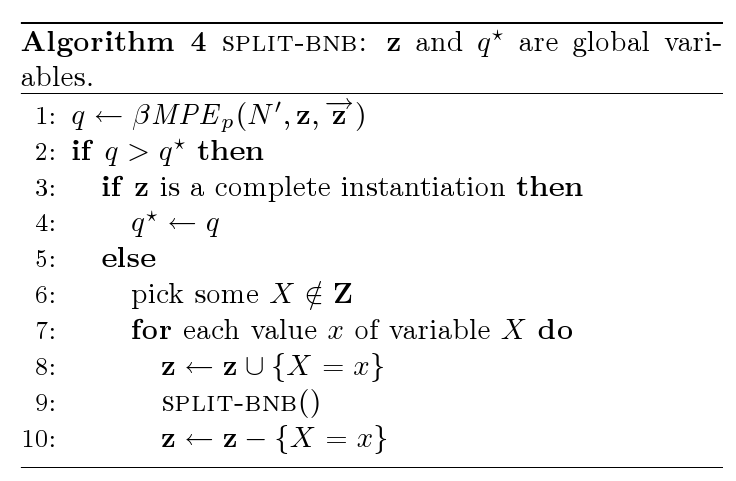
\includegraphics[width=24em]{splitbnb.png}\\
\end{center}

Llamemos a $L$ el conjunto de variables de $N$ a las que se le hizo
split. Un resultado importante de \cite{ChoiChaviraDarwiche07} es que
si todas las variables de $L$ están instanciadas entonces $MPE_p(N,
\mathbf{e}) = \beta MPE_p(N', \mathbf{e}, \vec{\mathbf{e}})$.
Como veremos en los resultados, ordenar los nodos para aprovechar esta propiedad
permite mejorar el proceso de búsqueda.

\section{Experimentos y resultados}

Para evaluar la calidad del software desarrollado lo ejecutamos sobre distintos
casos de prueba tomados de los casos usados en \cite{sangbeamekautzAAAI05}.
Todos los casos consistieron de \emph{grids} $N \times N$ de variables, con un
porcentaje especificado de nodos determinísticos. Por motivos de tiempo, el
conjunto de pruebas no fue tan exhaustivo como debería. Sin embargo, sí pudimos
obtener resultados preliminares que nos indican la calidad de las técnicas
implementadas.

Las redes utilizadas están nombradas con el formato \emph{R-N}, donde $R$ es el
porcentaje de nodos determinísticos y $N \times N$ el tamaño del grid.

\begin{table}
\begin{center}
  \begin{tabular}{l | l | l | l}
    \hline
    \#splits & 50-10 & 50-15 & 50-20 \\
    \hline
    20 & 9s & x & x \\
    50 & 8s & x & x \\
    75 & 13s & x & x \\
    100 & 17s & x & 2m23s \\
  \end{tabular}
  \caption{Tiempo de compilación a DNNF y creación de circuito según número de splits}
\end{center}
\end{table}

\section{Conclusiones}

Podemos nombrar varios logros alcanzados en el proyecto. En primer lugar
verificamos que la técnica de splitting puede influir fuertemente en el tiempo
de compilación a d-DNNF de fórmulas generadas por una red. Sin embargo,
hay un límite tras el cual hacer mucho splitting influye negativamente.
También vimos que hay
que balancear la velocidad de compilación deseada (mayor cuando hacemos más
splits) contra la velocidad del branch and bound (menor cuando hacemos más
splits).

La optimización basada en \emph{logical constraints} demostró su valor al
reducir enormemente el tiempo de compilación a d-DNNF. En
\cite{Darwiche01alogical} se explica que es una optimización que lleva a una
codificación más eficiente y que reduce dramáticamente el tamaño del d-DNNF
compilado al explotar restricciones lógicas a nivel de la codificación.
Nosotros pudimos comprobar esa
afirmación.

Por último, también pudimos observar mejoras en la velocidad del cálculo al
aplicar la heurística de ordenar los nodos para instanciar primero las variables
divididas en el branch and bound.

\section{Trabajo futuro}

Hay una optimización basada en \emph{context–specific independence} (CSI)
descrita en
\cite{Darwiche01alogical} junto con la optimización de \emph{logical constraints}
mencionada previamente. En resultados experimentales se ha mostrado que puede
tener un efecto importante de reducción del tamaño del d-DNNF y del circuito
aritmético resultantes de la compilación de una red bayesiana. Un paso natural a
seguir para la continuación de este proyecto es entonces ejecutar CSI sobre las
fórmulas CNF antes de su compilación con c2d.

Además, proponemos implementar el algoritmo de B\&B sobre la red en el
lenguaje \emph{C} (en vez de \emph{Python} como fue hecho) y prestando mayor
atención a la eficiencia del código. Creemos
que esto podría generar resultados aún mejores. En particular, pensamos en la
posibilidad de lograr el objetivo de calcular los MPE con la técnica descrita
para redes más grandes.

\bibliographystyle{plain}
\bibliography{informe}

\end{document}

%%% Local Variables: 
%%% mode: latex
%%% TeX-master: t
%%% End: 

